\documentclass[12pt]{article}

\usepackage{amsmath}
\usepackage{amssymb}
\usepackage{graphicx}
\usepackage{pifont}
\usepackage{listings}
\usepackage{xcolor}
\usepackage[T1]{fontenc}
\usepackage[utf8]{inputenc}
\usepackage{textcomp}
\usepackage{booktabs}
\usepackage{multirow}

\usepackage{pgf}
\usepackage{tikz}
\usetikzlibrary{arrows,automata}

\definecolor{listinggray}{gray}{0.9}
\definecolor{lbcolor}{rgb}{0.9,0.9,0.9}
\lstset{
	language=C++,
	frame = tb,
	numbers = left,
	showstringspaces = false,
	basicstyle=\ttfamily,
	keywordstyle=\color{blue}\ttfamily,
	stringstyle=\color{red}\ttfamily,
	commentstyle=\color{green}\ttfamily,
	morecomment=[l][\color{magenta}]{\#} 
}

\begin{document}

\begin{titlepage}
	\newcommand{\HRule}{\rule{\linewidth}{0.5mm}}
	
	\center
	
	\textsc{\Large Elektrotehnički fakultet Univerziteta Sarajevo}\\[4cm]
	
	{\huge\bfseries Diskretna Matematika\vspace{5mm}

 	Zadaća 3}\\[4.5cm]

	\begin{minipage}{0.4\textwidth}
		\begin{flushleft}
			\large
			\textit{Student}\\
			Vedad Fejzagić\\[5mm]
			\textit{Broj indeksa}\\
			17336\\[5mm]
			\textit{Grupa}\\
			RI2-2
		\end{flushleft}
	\end{minipage}
	~
	\begin{minipage}{0.4\textwidth}
		\begin{flushright}
			\large
			\textbf{Demonstrator}\\
			\hspace{10mm}Šeila Bečirović
		\end{flushright}
	\end{minipage}
	
	\vfill\vfill\vfill
	
	{\large\today}
	
	\vfill
	
\end{titlepage}


\newpage
\section*{Zadatak 1\label{Z1}}

\underline{Postavka:}

Neki eksperiment može dovesti do tri moguća događaja A1, A2 ili A3 iz skupa događaja X. Ova tri događaja imaju respektivno vjerovatnoće 0.25, 0.5 i 0.25. Rezultati tog eksperimenta nisu dostupni direktno, ali se može izvesti testni eksperiment koji daje događaje B1, B2, B3, B4 ili B5 iz skupa događaja Y, koji su u određenoj vezi sa događajima A1, A2 i A3. Vjerovatnoće da testni eksperiment rezultira događajem Bj, j = 1, 2, 3, 4, 5 ukoliko je izvorni eksperiment rezultirao događajem Ai, i = 1, 2, 3 date su u sljedećoj tabeli: 

\begin{table}[hp]
\centering
\begin{tabular}{|l|l|l|l|l|l|}
\hline
p($B_j$ / $A_i$) & $B_1$  & $B_2$  & $B_3$  & $B_4$  & $B_5$ \\ \hline
$A_1$          & 0.05 & 0.25 & 0.1  & 0.5  & 0.1 \\ \hline
$A_2$          & 0.15 & 0.35 & 0.05 & 0.35 & 0.1 \\ \hline
$A_3$          & 0.5  & 0.05 & 0.15 & 0.1  & 0.2 \\ \hline
\end{tabular}
\end{table}

Odredite entropije skupa izvornih i testnih događaja H(X) i H(Y), uvjetne entropije H(X/Y) i H(Y/X), zajedničku entropiju H(X,Y) te srednju količinu informacije I(X,Y) koju testni događaji nose o izvornim događajima.

\underline{Rješenje:}\\


$$H(X) = - \frac{1}{ln 2} \cdot (0.25 \ln{0.25} + 0.5 \ln{0.5} + 0.25 \ln{0.25}) = 1.5$$

Računamo vrijednosti $p(B_j)$ za $j = 1, 2, 3, 4, 5$:

$$p(B_j) = \sum_{i = 1}^{3} p(A_i) \cdot p(B_j / A_i)$$

Dobijamo:

$$p(B_1) = p(A_1) p(B_1 / A_1) + p(A_2) p(B_1 / A_2) + p(A_3) p(B_1 / A_3) = 0.2125$$
$$p(B_2) = 0.25$$
$$p(B_3) = 0.0875$$
$$p(B_4) = 0.325$$
$$p(B_5) = 0.125$$

$$H(Y) =  - \frac{1}{ln 2} \cdot (0.2125 \ln{0.2125} + 0.25 \ln{0.25} +$$ 
$$+ 0.0875 \ln{0.0875} + 0.325 \ln{0.325}  + 0.125 \ln{0.125}) = 2.178432$$

Sada računamo $p(A_i B_j)$, za $i = 1. 2. 3 ; j = 1, 2, 3, 4, 5$ Rezultati prikazani u vidu tabele:

\begin{table}[hp]
\centering
\begin{tabular}{|l|l|l|l|l|l|}
\hline
p($A_i$ $B_j$) & $B_1$    & $B_2$    & $B_3$    & $B_4$   & $B_5$   \\ \hline
$A_1$          & 0.0125 & 0.0625 & 0.025  & 0.125 & 0.025 \\ \hline
$A_2$          & 0.075  & 0.175  & 0.025  & 0.175 & 0.05  \\ \hline
$A_3$         & 0.125  & 0.0125 & 0.0375 & 0.025 & 0.05  \\ \hline
\end{tabular}
\end{table}

$$H(X, Y) = - \sum_{i = 1}^{3} \sum_{j = 1}^{5} p(A_i B_j) \cdot \log_2 p(A_i B_j)$$
$$H(X, Y) = - \frac{1}{\ln{2}} \sum_{i = 1}^{3} \sum_{j = 1}^{5} p(A_i B_j) \cdot \ln{p(A_i B_j)}$$
$$H(X, Y) = 3.4604$$

$$H(X / Y) = H(X, Y) - H(Y) = 1.27608$$
$$H(Y / X) = H(X, Y) - H(X) = 1.9604$$
$$I(X, Y) = H(X) + H(Y) - H(X, Y) = 0.218$$

\newpage

\section*{Zadatak 2\label{Z2}}

\underline{Postavka:}

Na nekom fakultetu, troškove studija za 22\% studenata plaća država, dok su ostali studenti samofinansirajući. Među studentima koji se školuju o trošku države, 47\% studenata stanuje u studentskom domu, dok među samofinansirajućim studentima 32\% studenata stanuje u studentskom domu. Svi studenti koji stanuju u studentskom domu ujedno posjeduju i iskaznicu za subvencionirani javni prevoz, dok među studentima koji ne stanuju u studentskom domu istu iskaznicu posjeduje i 32\% studenata čiji studij plaća država te 40\% samofinansirajućih studenata.\\

Odredite koliku prosječnu količinu informacije saznanje o tome posjeduje li student iskaznicu za subvencionirani javni prenos ili ne nosi o načinu finansiranja njegovog studija (tj. da li ga finansira država ili troškove snosi sam).

\underline{Rješenje:}\\


\newpage

\section*{Zadatak 3\label{Z3}}

\underline{Postavka:}

Markovljev izvor informacija prvog reda emitira četiri različite poruke a, b, c i d. Ovisno od toga koja je poruka posljednja emitirana, izvor se nalazi u jednom od 4 moguća stanja Sa, Sb, Sc i Sd koja redom odgovaraju emitiranim porukama a, b, c odnosno d. Vjerovatnoće da će izvor emitirati neku od ove 4 poruke ovisno od stanja u kojem se nalazi date su u sljedećoj tablici: 

\begin{table}[hp]
\centering
\begin{tabular}{|l|l|l|l|l|}
\hline
p($x_j$ / $S_i$) & a    & b    & c    & d    \\ \hline
$S_a$           & 0.4  & 0.15 & 0.3  & 0.15 \\ \hline
$S_b$           & 0.4  & 0.4  & 0.1  & 0.1  \\ \hline
$S_c$           & 0.05 & 0.35 & 0.1  & 0.5  \\ \hline
$S_d$           & 0.3  & 0.1  & 0.45 & 0.15 \\ \hline
\end{tabular}
\end{table}

Odredite entropiju i redudansu ovog izvora, zatim entropiju sekvenci dužine 6 te vjerovatnoću pojave sekvence aaabdb.

\underline{Rješenje:}\\

Red izvora je r = 1, izvor modeliramo pomoću 4 stanja:

\begin{center}
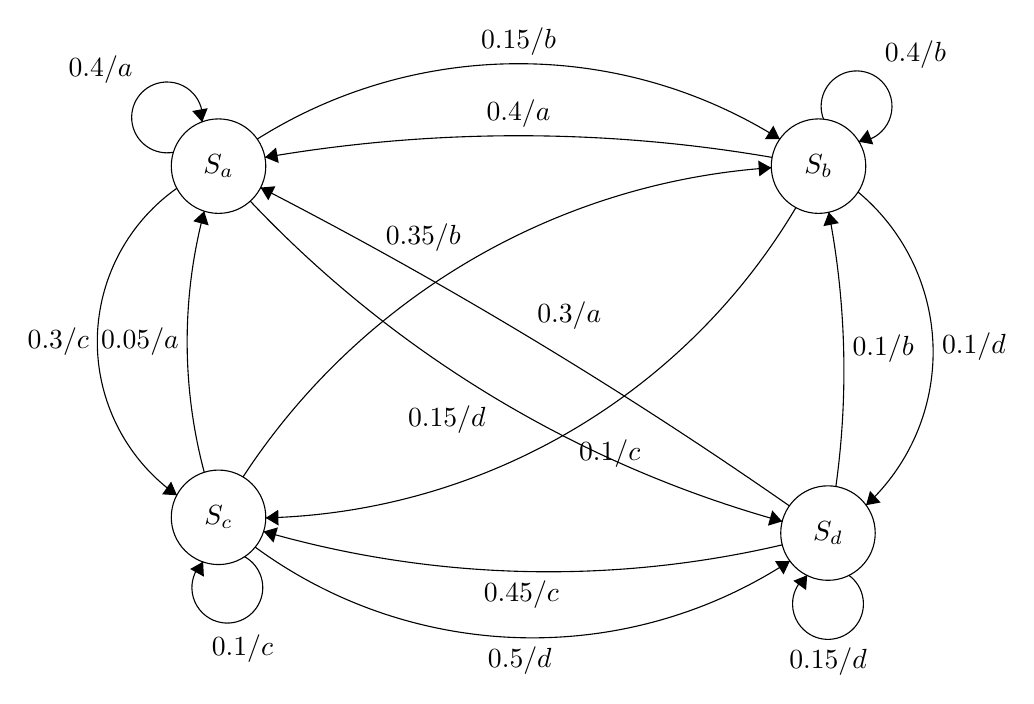
\begin{tikzpicture}[scale=0.2]
\tikzstyle{every node}+=[inner sep=0pt]
\draw [black] (19.5,-16.4) circle (3);
\draw (19.5,-16.4) node {$S_a$};
\draw [black] (57.6,-16.4) circle (3);
\draw (57.6,-16.4) node {$S_b$};
\draw [black] (19.5,-38.7) circle (3);
\draw (19.5,-38.7) node {$S_c$};
\draw [black] (58.2,-39.7) circle (3);
\draw (58.2,-39.7) node {$S_d$};
\draw [black] (21.958,-14.682) arc (122.18765:57.81235:31.147);
\fill [black] (55.14,-14.68) -- (54.73,-13.83) -- (54.2,-14.68);
\draw (38.55,-9.4) node [above] {$0.15/b$};
\draw [black] (22.448,-15.844) arc (99.76857:80.23143:94.903);
\fill [black] (22.45,-15.84) -- (23.32,-16.2) -- (23.15,-15.22);
\draw (38.55,-13.97) node [above] {$0.4/a$};
\draw [black] (16.645,-15.517) arc (280.54816:-7.45184:2.25);
\draw (14.07,-10.29) node [left] {$0.4/a$};
\fill [black] (18.46,-13.6) -- (18.81,-12.72) -- (17.83,-12.9);
\draw [black] (21.145,-41.195) arc (61.12502:-226.87498:2.25);
\draw (21.02,-46.12) node [below] {$0.1/c$};
\fill [black] (18.52,-41.52) -- (17.7,-41.98) -- (18.57,-42.47);
\draw [black] (59.523,-42.38) arc (54:-234:2.25);
\draw (58.2,-46.95) node [below] {$0.15/d$};
\fill [black] (56.88,-42.38) -- (56,-42.73) -- (56.81,-43.32);
\draw [black] (57.923,-13.429) arc (201.52881:-86.47119:2.25);
\draw (63.75,-10.2) node [above] {$0.4/b$};
\fill [black] (60.15,-14.85) -- (61.08,-15.02) -- (60.72,-14.09);
\draw [black] (16.857,-37.297) arc (-125.17132:-234.82868:11.924);
\fill [black] (16.86,-37.3) -- (16.49,-36.43) -- (15.92,-37.24);
\draw (11.3,-27.55) node [left] {$0.3/c$};
\draw [black] (18.593,-35.841) arc (-165.06887:-194.93113:32.18);
\fill [black] (18.59,-19.26) -- (17.9,-19.9) -- (18.87,-20.16);
\draw (17.01,-27.55) node [left] {$0.05/a$};
\draw [black] (55.779,-41.47) arc (-56.71755:-126.24281:29.784);
\fill [black] (55.78,-41.47) -- (54.84,-41.49) -- (55.38,-42.33);
\draw (38.63,-46.91) node [below] {$0.5/d$};
\draw [black] (55.295,-40.449) arc (-76.85012:-106.11025:65.216);
\fill [black] (22.36,-39.6) -- (22.99,-40.3) -- (23.27,-39.34);
\draw (38.73,-42.71) node [below] {$0.45/c$};
\draw [black] (58.251,-19.328) arc (10.91558:-7.96538:53.102);
\fill [black] (58.25,-19.33) -- (57.91,-20.21) -- (58.89,-20.02);
\draw (59.73,-28.01) node [right] {$0.1/b$};
\draw [black] (60.104,-18.04) arc (50.27352:-47.32331:13.224);
\fill [black] (60.62,-37.93) -- (61.54,-37.76) -- (60.87,-37.02);
\draw (65.41,-27.86) node [right] {$0.1/d$};
\draw [black] (55.293,-38.958) arc (-105.49551:-136.60602:73.512);
\fill [black] (55.29,-38.96) -- (54.66,-38.26) -- (54.39,-39.23);
\draw (33.99,-31.6) node [below] {$0.15/d$};
\draw [black] (22.174,-17.759) arc (62.76788:55.13059:294.212);
\fill [black] (22.17,-17.76) -- (22.66,-18.57) -- (23.11,-17.68);
\draw (41.77,-26.8) node [above] {$0.3/a$};
\draw [black] (21.054,-36.135) arc (146.81953:93.8615:43.591);
\fill [black] (54.6,-16.5) -- (53.77,-16.05) -- (53.84,-17.05);
\draw (32.5,-21.87) node [above] {$0.35/b$};
\draw [black] (56.163,-19.033) arc (-30.75497:-88.56399:40.35);
\fill [black] (22.5,-38.74) -- (23.31,-39.22) -- (23.29,-38.22);
\draw (44.34,-33.73) node [below] {$0.1/c$};
\end{tikzpicture}
\end{center}

Računamo vjerovatnoće za svako od stanja rješavanjem sljedećeg sistema jednačina:

$$p(S_a) = p(S_a) p(a/S_a) + p(S_b) p(a/S_b) + p(S_c) p(a/S_c) + p(S_d) p(a/S_d)$$
$$p(S_b) = p(S_a) p(b/S_a) + p(S_b) p(b/S_b) + p(S_c) p(b/S_c) + p(S_d) p(b/S_d)$$
$$p(S_c) = p(S_a) p(c/S_a) + p(S_b) p(c/S_b) + p(S_c) p(c/S_c) + p(S_d) p(c/S_d)$$
$$p(S_a) + p(S_b) + p(S_c) + p(S_d) = 1$$

Nakon uvrštavanja vrijednosti i prebacivanja $p(S_a), p(S_b), p(S_c)$ na desnu stranu jednakosti, dobijamo sljedeću matricu:

\[
M=
  \begin{bmatrix}
    -0.6 & 0.4 & 0.05 & 0.3 & | 0 \\
    0.15 & -0.6 & 0.35 & 0.1 & | 0 \\
	0.3 & 0.1 & -0.9 & 0.45 & | 0 \\
	1 & 1 & 1 & 1 & | 1
  \end{bmatrix}
\]

Koristimo Gausov metod eliminacije da riješimo zadani sistem, svođenjem matrice na desnu trougaonu matricu, dobijamo:

\[
M=
  \begin{bmatrix}
    -0.6	& 0.4	&0.05	&0.3 & | 0 \\
	0 &	-0.5&	0.36&	0.17& |	0\\
	0 &	0	&-0.65&	0.70& |	0\\
	0	&0	&0	&4.54 &| 1
  \end{bmatrix}
\]

$$-0.6p(S_a) + 0.4p(S_b) + 0.05p(S_c) + 0.3p(S_d) = 0$$
$$-0.5p(S_b) + 0.36p(S_c) + 0.17p(S_d) = 0$$
$$-0.65p(S_c) + 0.70p(S_d) = 0$$
$$ 4.54p(S_d) = 1$$
 
Dakle, rješenja sistema su:

$$p(S_a) = 0.29$$
$$p(S_b) = 0.25$$
$$p(S_c) = 0.23$$
$$p(S_d) = 0.22$$


$$H(S_a) = - \frac{1}{\ln{2}} (p(a/S_a) \ln{p(a/S_a)} + p(b/S_a) \ln{p(b/S_a)} + p(c/S_a) \ln{p(c/S_a)} + p(d/S_a) \ln{p(d/S_a)})$$

Analogno za ostale, dobijamo: 

$$H(S_a) \approx 1.871$$
$$H(S_b) \approx 1.722$$
$$H(S_c) \approx 1.578$$
$$H(S_d) \approx 1.782$$

$$H(X/X^{\infty}) = \sum_{i = 1}^{4} p(S_i) H(S_i) = 1.73$$
$$H_{max} = \log_{2}4 = \frac{\ln{4}}{\ln{2}} = 2$$

$$R = \frac{H_{max} - H(X/X^{\infty})}{H_{max}} \approx 0.135 = 13.5\%$$

$$H(X) = - \frac{1}{\ln{2}} (p(a) \ln{p(a)} + p(b) \ln{p(b)} + p(c) \ln{p(c)} + p(d) \ln{p(d)}) \approx 1.98614$$

$$H(X^6) = H(X) + (6 - 1) H(X / X^{\infty}) \approx 10.636$$

$$p(aaabdb) = p(a) p(a/a) p(a/a) p(b/a) p(d/b) p(b/d) = 0.0000696 = 0.00696\%$$


\newpage

\section*{Zadatak 4\label{Z4}}

\underline{Postavka:}

Markovljev izvor informacija drugog reda emitira dvije različite poruke 0 i 1. Ovisno od toga koje su dvije poruke posljednje emitirane, izvor se može naći u jednom od 4 moguća stanja S00, S01, S10 odnosno S11 (recimo, ukoliko su posljednje dvije emitirane poruke 0 i 1 tim redom, izvor će se nalaziti u stanju S01). Vjerovatnoće emitiranja poruke 0 u svakom od tih stanja iznose:

$$p(0/S_{00}) = 0.9$$
$$p(0/S_{01}) = 0.7$$
$$p(0/S_{10}) = 0.1$$
$$p(0/S_{11}) = 0.2$$

Odredite entropiju i redudansu ovog izvora, zatim entropiju sekvenci dužine 6 te vjerovatnoću pojave sekvence 00101100.

\underline{Rješenje:}\\

$$p(0/S_{00}) = 0.9, p(1/S_{00}) = 0.1$$

$$p(0/S_{01}) = 0.7, p(1/S_{01}) = 0.3$$

$$p(0/S_{10}) = 0.1, p(1/S_{10}) = 0.9$$

$$p(0/S_{11}) = 0.2, p(1/S_{11}) = 0.8$$\\

Neka su $S_{00} = S_1$, $S_{01} = S_2$, $S_{10} = S_3$, $S_{11} = S_4$.

\begin{center}
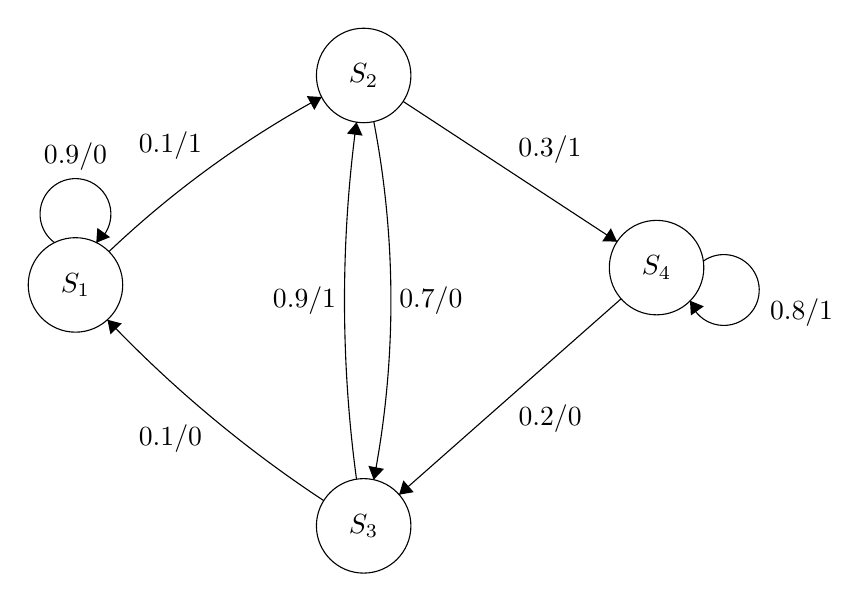
\begin{tikzpicture}[scale=0.2]
\tikzstyle{every node}+=[inner sep=0pt]
\draw [black] (22,-26.9) circle (3);
\draw (22,-26.9) node {$S_1$};
\draw [black] (58.9,-25.8) circle (3);
\draw (58.9,-25.8) node {$S_4$};
\draw [black] (40.3,-13.6) circle (3);
\draw (40.3,-13.6) node {$S_2$};
\draw [black] (40.3,-42.2) circle (3);
\draw (40.3,-42.2) node {$S_3$};
\draw [black] (20.677,-24.22) arc (234:-54:2.25);
\draw (22,-19.65) node [above] {$0.9/0$};
\fill [black] (23.32,-24.22) -- (24.2,-23.87) -- (23.39,-23.28);
\draw [black] (24.126,-24.784) arc (133.5123:118.50521:63.921);
\fill [black] (37.63,-14.97) -- (36.69,-14.91) -- (37.17,-15.79);
\draw (28.03,-18.94) node [above] {$0.1/1$};
\draw [black] (37.765,-40.597) arc (-123.39807:-136.3976:79.091);
\fill [black] (24.03,-29.11) -- (24.22,-30.04) -- (24.94,-29.35);
\draw (28.03,-35.74) node [below] {$0.1/0$};
\draw [black] (39.845,-39.235) arc (-172.30061:-187.69939:84.603);
\fill [black] (39.85,-16.57) -- (39.24,-17.29) -- (40.23,-17.42);
\draw (38.58,-27.9) node [left] {$0.9/1$};
\draw [black] (40.943,-16.53) arc (10.94937:-10.94937:59.861);
\fill [black] (40.94,-39.27) -- (41.59,-38.58) -- (40.6,-38.39);
\draw (42.53,-27.9) node [right] {$0.7/0$};
\draw [black] (42.81,-15.25) -- (56.39,-24.15);
\fill [black] (56.39,-24.15) -- (56,-23.3) -- (55.45,-24.13);
\draw (52.13,-19.2) node [above] {$0.3/1$};
\draw [black] (56.65,-27.78) -- (42.55,-40.22);
\fill [black] (42.55,-40.22) -- (43.48,-40.06) -- (42.82,-39.31);
\draw (52.14,-34.49) node [below] {$0.2/0$};
\draw [black] (61.86,-25.393) arc (125.56505:-162.43495:2.25);
\draw (66.07,-28.64) node [right] {$0.8/1$};
\fill [black] (61.02,-27.9) -- (61.08,-28.84) -- (61.9,-28.26);
\end{tikzpicture}
\end{center}


Potrebne su nam vrijednosti $p(S_1), p(S_2), p(S_3), p(S_4)$

$$p(S_1) = p(S_1) p(0/S_1) + p(S_3) p(0/S_3)$$
$$0.1 p(S_1) = 0.1 p(S_3)$$
$$p(S_1) = p(S_3)$$

Analogno za ostale, dobije se:

$$p(S_2) = p(S_3)$$
$$0.3 p(S_3) = 0.2 p(S_4)$$

Potrebno je riješiti sljedeći sistem:
$$p(S_1) = p(S_3)$$
$$p(S_2) = p(S_3)$$
$$0.3 p(S_3) = 0.2 p(S_4)$$
$$p(S_1) + p(S_2)  + p(S_3) + p(S_4) = 1$$

Rješavanjem sistema, dobiju se sljedeće vrijednosti:

$$p(S_1) = 0.2222$$
$$p(S_2) = 0.2222$$
$$p(S_3) = 0.2222$$
$$p(S_4) = 0.3333$$

$$H(S_1) = - \frac{1}{\ln{2}} (p(0/S_1) \ln{p(0/S_1)} + p(1/S_1) \ln{p(1/S_1)}) \approx 0.47$$
$$H(S_2) \approx 0.881291$$
$$H(S_3) \approx 0.468996$$
$$H(S_4) \approx 0.721928$$

$$H(X/X^{\infty}) = \sum_{i = 1}^{4} p(S_i) H(S_i) = 0.638$$

Redudansa:

$$H_{max} = \log_{2}4 = 2$$
$$R = \frac{H_{max} - H(X/X^{\infty})}{H_{max}} \approx 0.681 \approx 68.1 \%$$ \\

Entropija sekvenci dužine 6:

$$H(X^2) = - \frac{1}{\ln{2}} (p(00) \ln{p(00)} + p(01) \ln{p(01)} + p(10) \ln{p(10)} + p(11) \ln{p(11)}) = 1.96954$$

$$H(X^6) = H(X^2) + 4  H(X/X^{\infty}) \approx 4.52154$$\\

Vjerovatnoća pojave sekvence 00101100:

$$p(00101100) = p(00) p(1/00)p(0/01)p(1/10)p(1/01)p(0/11)p(0/10) = 0.00008316 = 0.008316\%$$


\newpage

\section*{Zadatak 5\label{Z5}}

\underline{Postavka:}

Ergodični izvor informacija bez memorije emitira 10 poruka A, B, C, D, E, F, G, H, I i J. Proučavanjem sekvence dužine 645 koju je emitirao ovaj izvor, uočena je sljedeća učestalost pojavljivanja pojedinih poruka: 

\begin{table}[hp]
\centering
\begin{tabular}{|l|l|l|l|l|l|l|l|l|l|l|}
\hline
Poruka:     & A  & B  & C  & D  & E  & F  & G  & H  & I  & J  \\ \hline
Učestalost: & 18 & 73 & 87 & 49 & 73 & 99 & 98 & 44 & 80 & 24 \\ \hline
\end{tabular}
\end{table}

Za ovaj izvor informacija formirajte:

a) Binarni Shannon-Fano kod sa simbolima 0 i 1;

b) Binarni Huffmanov kod sa simbolima 0 i 1;

c) Ternarni Huffmanov kod sa simbolima 0, 1 i 2.

Za sva tri načina kodiranja, izračunajte protok informacija kroz komunikacioni kanal, procenat iskorištenja kanala veze, te kodirajte sekvencu poruka BAIBBBJIDJCE.

\underline{Rješenje:}\\

a)\\

Sortiramo:

\begin{table}[hp]
\centering
\begin{tabular}{|l|l|}
\hline
F & 99 \\ \hline
G & 98 \\ \hline
C & 87 \\ \hline
I & 80 \\ \hline
B & 73 \\ \hline
E & 73 \\ \hline
D & 49 \\ \hline
H & 44 \\ \hline
J & 24 \\ \hline
A & 18 \\ \hline
\end{tabular}
\end{table}

Kodiramo pomoću binarnog stabla:

\begin{center}
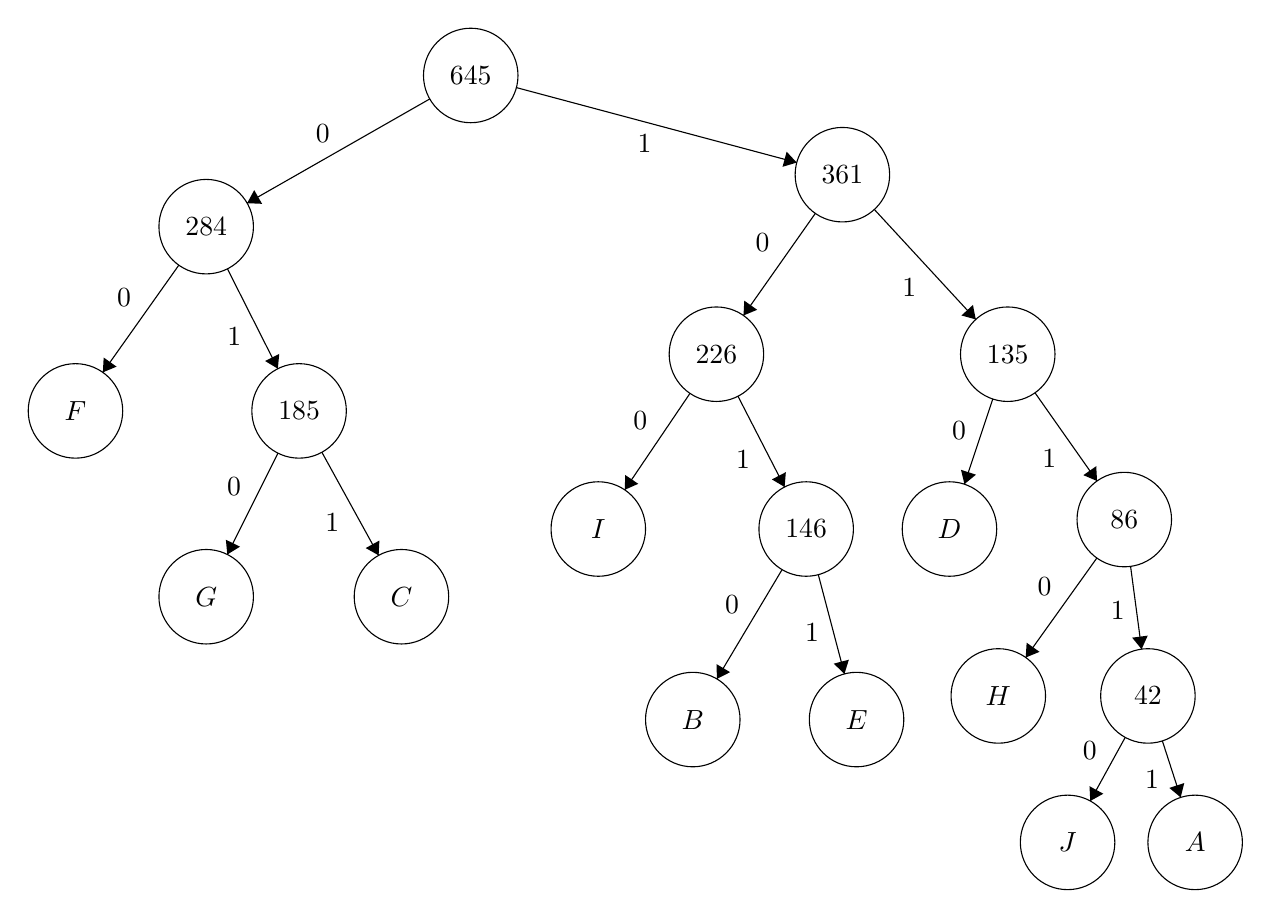
\begin{tikzpicture}[scale=0.2]
\tikzstyle{every node}+=[inner sep=0pt]
\draw [black] (30.9,-5.6) circle (3);
\draw (30.9,-5.6) node {$645$};
\draw [black] (14.1,-15.2) circle (3);
\draw (14.1,-15.2) node {$284$};
\draw [black] (54.5,-11.9) circle (3);
\draw (54.5,-11.9) node {$361$};
\draw [black] (5.8,-26.9) circle (3);
\draw (5.8,-26.9) node {$F$};
\draw [black] (20,-26.9) circle (3);
\draw (20,-26.9) node {$185$};
\draw [black] (14.1,-38.7) circle (3);
\draw (14.1,-38.7) node {$G$};
\draw [black] (26.5,-38.7) circle (3);
\draw (26.5,-38.7) node {$C$};
\draw [black] (46.5,-23.3) circle (3);
\draw (46.5,-23.3) node {$226$};
\draw [black] (65,-23.3) circle (3);
\draw (65,-23.3) node {$135$};
\draw [black] (39,-34.4) circle (3);
\draw (39,-34.4) node {$I$};
\draw [black] (52.2,-34.4) circle (3);
\draw (52.2,-34.4) node {$146$};
\draw [black] (45,-46.5) circle (3);
\draw (45,-46.5) node {$B$};
\draw [black] (55.4,-46.5) circle (3);
\draw (55.4,-46.5) node {$E$};
\draw [black] (61.3,-34.4) circle (3);
\draw (61.3,-34.4) node {$D$};
\draw [black] (72.4,-33.8) circle (3);
\draw (72.4,-33.8) node {$86$};
\draw [black] (64.4,-45) circle (3);
\draw (64.4,-45) node {$H$};
\draw [black] (73.9,-45) circle (3);
\draw (73.9,-45) node {$42$};
\draw [black] (68.8,-54.3) circle (3);
\draw (68.8,-54.3) node {$J$};
\draw [black] (76.9,-54.3) circle (3);
\draw (76.9,-54.3) node {$A$};
\draw [black] (28.3,-7.09) -- (16.7,-13.71);
\fill [black] (16.7,-13.71) -- (17.65,-13.75) -- (17.15,-12.88);
\draw (21.5,-9.9) node [above] {$0$};
\draw [black] (33.8,-6.37) -- (51.6,-11.13);
\fill [black] (51.6,-11.13) -- (50.96,-10.44) -- (50.7,-11.4);
\draw (41.94,-9.31) node [below] {$1$};
\draw [black] (12.36,-17.65) -- (7.54,-24.45);
\fill [black] (7.54,-24.45) -- (8.41,-24.09) -- (7.59,-23.51);
\draw (9.36,-19.68) node [left] {$0$};
\draw [black] (15.45,-17.88) -- (18.65,-24.22);
\fill [black] (18.65,-24.22) -- (18.74,-23.28) -- (17.84,-23.73);
\draw (16.36,-22.16) node [left] {$1$};
\draw [black] (18.66,-29.58) -- (15.44,-36.02);
\fill [black] (15.44,-36.02) -- (16.25,-35.52) -- (15.35,-35.08);
\draw (16.35,-31.69) node [left] {$0$};
\draw [black] (21.45,-29.53) -- (25.05,-36.07);
\fill [black] (25.05,-36.07) -- (25.1,-35.13) -- (24.23,-35.61);
\draw (22.58,-33.99) node [left] {$1$};
\draw [black] (52.78,-14.36) -- (48.22,-20.84);
\fill [black] (48.22,-20.84) -- (49.09,-20.48) -- (48.27,-19.9);
\draw (49.9,-16.24) node [left] {$0$};
\draw [black] (56.53,-14.11) -- (62.97,-21.09);
\fill [black] (62.97,-21.09) -- (62.79,-20.17) -- (62.06,-20.84);
\draw (59.22,-19.06) node [left] {$1$};
\draw [black] (44.82,-25.79) -- (40.68,-31.91);
\fill [black] (40.68,-31.91) -- (41.54,-31.53) -- (40.71,-30.97);
\draw (42.14,-27.51) node [left] {$0$};
\draw [black] (47.87,-25.97) -- (50.83,-31.73);
\fill [black] (50.83,-31.73) -- (50.91,-30.79) -- (50.02,-31.25);
\draw (48.66,-29.98) node [left] {$1$};
\draw [black] (50.67,-36.98) -- (46.53,-43.92);
\fill [black] (46.53,-43.92) -- (47.37,-43.49) -- (46.51,-42.98);
\draw (47.96,-39.19) node [left] {$0$};
\draw [black] (52.97,-37.3) -- (54.63,-43.6);
\fill [black] (54.63,-43.6) -- (54.91,-42.7) -- (53.95,-42.95);
\draw (53.04,-40.95) node [left] {$1$};
\draw [black] (64.05,-26.15) -- (62.25,-31.55);
\fill [black] (62.25,-31.55) -- (62.98,-30.95) -- (62.03,-30.64);
\draw (62.38,-28.15) node [left] {$0$};
\draw [black] (66.73,-25.75) -- (70.67,-31.35);
\fill [black] (70.67,-31.35) -- (70.62,-30.41) -- (69.8,-30.98);
\draw (68.11,-29.92) node [left] {$1$};
\draw [black] (70.66,-36.24) -- (66.14,-42.56);
\fill [black] (66.14,-42.56) -- (67.02,-42.2) -- (66.2,-41.62);
\draw (67.81,-38.03) node [left] {$0$};
\draw [black] (72.8,-36.77) -- (73.5,-42.03);
\fill [black] (73.5,-42.03) -- (73.89,-41.17) -- (72.9,-41.3);
\draw (72.47,-39.55) node [left] {$1$};
\draw [black] (72.46,-47.63) -- (70.24,-51.67);
\fill [black] (70.24,-51.67) -- (71.07,-51.21) -- (70.19,-50.73);
\draw (70.68,-48.46) node [left] {$0$};
\draw [black] (74.82,-47.86) -- (75.98,-51.44);
\fill [black] (75.98,-51.44) -- (76.21,-50.53) -- (75.26,-50.84);
\draw (74.63,-50.32) node [left] {$1$};
\end{tikzpicture}
\end{center}

Kodirane poruke su sljedeće:

\begin{table}[hp]
\centering
\begin{tabular}{|l|l|}
\hline
F & 00    \\ \hline
G & 010   \\ \hline
C & 011   \\ \hline
I & 100   \\ \hline
B & 1010  \\ \hline
E & 1011  \\ \hline
D & 110   \\ \hline
H & 1110  \\ \hline
J & 11110 \\ \hline
A & 11111 \\ \hline
\end{tabular}
\end{table}

Kodirana sekvenca poruka: BAIBBBJIDJCE glasi:

$$10101111110010101010101011110100110111100111011$$

Prosječna dužina kodne riječi: 

$$n_{sr} = \sum_{i = 1}^{10} p_i n_i \approx \sum_{i = 1}^{10} \frac{N_i}{N} n_i = \frac{1}{N} \sum_{i = 1}^{10} N_i n_i$$
$$n_{sr} = 3.271$$

Entropija izvora:

$$H(X/X^{\infty}) = H(X) =  - \sum_{i = 1}^{10} p_i \log_{2}p_i = ... = \frac{1}{\ln{2}} (\ln{N} - \frac{1}{N} \sum_{i = 1}^{10} N_i \ln{N_i})$$
$$H(X/X^{\infty}) = 3.1671$$

Protok informacija:

$$\overline{I(H)} = \frac{H(X/X^{\infty}) }{n_{sr} \tau} \approx \frac{0.968}{\tau}$$

Iskorištenost kanala veze 96.8\%

b)\\

Iz postavke: $n = 10, m = 2 \to m^{*} = 2 + mod(n - 4, m - 1) = 2$
Prelazimo na formiranje binarnog Huffmanovog koda:
\newpage
\begin{table}[hp]
\hspace*{-1.0in}
\begin{tabular}{|l|l|l|l|l|l|l|l|l|l|l|l|l|l|l|l|}
\hline
\multicolumn{2}{|l|}{Početak} & \multicolumn{2}{l|}{Iteracija 1}               & \multicolumn{2}{l|}{Iteracija 2} & \multicolumn{2}{l|}{Iteracija 3} & \multicolumn{2}{l|}{Iteracija 4} & \multicolumn{2}{l|}{Iteracija 5} & \multicolumn{2}{l|}{Iteracija 6} & \multicolumn{2}{l|}{Iteracija 7} \\ \hline
F             & 99            & F   & 99                                       & F       & 99                     & E/0     & \multirow{2}{*}{122}   & I/0     & \multirow{2}{*}{153}   & C/0     & \multirow{4}{*}{173}   & F/0     & \multirow{2}{*}{197}   & I/00    & \multirow{4}{*}{275}   \\ \cline{1-6}
G             & 98            & G   & 98                                       & G       & 98                     & D/1     &                        & B/1     &                        & H/10    &                        & G/1     &                        & B/01    &                        \\ \cline{1-10} \cline{13-14}
C             & 87            & C   & 87                                       & C       & 87                     & F       & 99                     & E/0     & \multirow{2}{*}{122}   & J/110   &                        & C/0     & \multirow{4}{*}{173}   & E/10    &                        \\ \cline{1-8}
I             & 80            & I   & 80                                       & H/0     & \multirow{3}{*}{86}    & G       & 98                     & D/1     &                        & A/111   &                        & H/10    &                        & D/11    &                        \\ \cline{1-4} \cline{7-12} \cline{15-16} 
B             & 73            & B   & 73                                       & J/10    &                        & C       & 87                     & F       & 99                     & I/0     & \multirow{2}{*}{153}   & J/110   &                        & F/0     & \multirow{2}{*}{197}   \\ \cline{1-4} \cline{7-10}
E             & 73            & E   & 73                                       & A/11    &                        & H/0     & \multirow{3}{*}{86}    & G       & 98                     & B/1     &                        & A/111   &                        & G/1     &                        \\ \cline{1-6} \cline{9-16} 
D             & 49            & D   & 49                                       & I       & 80                     & J/10    &                        & C       & 87                     & E/0     & \multirow{2}{*}{122}   & I/0     & \multirow{2}{*}{153}   & C/0     & \multirow{4}{*}{173}   \\ \cline{1-6} \cline{9-10}
H             & 44            & H   & 44                                       & B       & 73                     & A/11    &                        & H/0     & \multirow{3}{*}{86}    & D/1     &                        & B/1     &                        & H/10    &                        \\ \cline{1-8} \cline{11-14}
J             & 24            & J/0 & \multicolumn{1}{c|}{\multirow{2}{*}{42}} & E       & 73                     & I       & 80                     & J/10    &                        & F       & 99                     & E/0     & \multirow{2}{*}{122}   & J/110   &                        \\ \cline{1-2} \cline{5-8} \cline{11-12}
A             & 18            & A/1 & \multicolumn{1}{c|}{}                    & D       & 49                     & B       & 73                     & A/11    &                        & G       & 98                     & D/1     &                        & A/111   &                        \\ \hline
\end{tabular}
\end{table}

\begin{table}[hp]
\centering
\begin{tabular}{|l|l|l|l|}
\hline
\multicolumn{2}{|l|}{Iteracija 8} & \multicolumn{2}{l|}{Iteracija 9} \\ \hline
F/00 & \multirow{6}{*}{370} & I/000 & \multirow{10}{*}{645} \\
G/01 &  & G/001 &  \\
C/10 &  & C/010 &  \\
H/110 &  & H/0110 &  \\
J/1110 &  & J/01110 &  \\
A/1111 &  & A/01111 &  \\ \cline{1-2}
I/00 & \multirow{4}{*}{275} & I/100 &  \\
B/01 &  & B/101 &  \\
E/10 &  & E/110 &  \\
D/11 &  & D/111 &  \\ \hline
\end{tabular}
\end{table}

\textit{U sljedecim zadacima koji zahtjevaju veci broj iteracija, nece citav postupak biti prikazan}

$$n_{sr} = \frac{1}{645} (\sum_{i = 1}^{10} N_i n_i) = 3.271$$
$$\overline{I(X)} = \frac{H(X/X^{\infty}) }{n_{sr} \tau} \approx \frac{0.968}{\tau}$$

Iskorištenost kanala veze 96.8\%.

Kodirana sekvenca poruka: BAIBBBJIDJCE glasi:

$$101011111001011011010111010011101110010110$$

c)\\

Ternarni Huffmanov kod: $m = 0, m^{*} = 2 + mod(6, 2) = 2$

\begin{table}[hp]
\centering
\begin{tabular}{|l|l|l|l|l|l|l|l|l|l|l|l|}
\hline
\multicolumn{2}{|l|}{Početak} & \multicolumn{2}{l|}{Iteracija 1} & \multicolumn{2}{l|}{Iteracija 2} & \multicolumn{2}{l|}{Iteracija 3} & \multicolumn{2}{l|}{Iteracija 4} & \multicolumn{2}{l|}{Iteracija 5} \\ \hline
F             & 99            & F       & 99                     & D/0     & \multirow{4}{*}{135}   & I/0     & \multirow{3}{*}{226}   & F/0     & \multirow{3}{*}{284}   & F/00    & \multirow{10}{*}{645}  \\ \cline{1-4}
G             & 98            & G       & 98                     & H/1     &                        & B/1     &                        & G/1     &                        & G/01    &                        \\ \cline{1-4}
C             & 87            & C       & 87                     & J/20    &                        & E/2     &                        & C/2     &                        & C/02    &                        \\ \cline{1-4} \cline{7-10}
I             & 80            & I       & 80                     & A/21    &                        & D/0     & \multirow{4}{*}{135}   & I/0     & \multirow{3}{*}{226}   & I/10    &                        \\ \cline{1-6}
B             & 73            & B       & 73                     & F       & 99                     & H/1     &                        & B/1     &                        & B/11    &                        \\ \cline{1-6}
E             & 73            & E       & 73                     & G       & 98                     & J/20    &                        & E/2     &                        & E/12    &                        \\ \cline{1-6} \cline{9-10}
D             & 49            & D       & 49                     & C       & 87                     & A/21    &                        & D/0     & \multirow{4}{*}{135}   & D/20    &                        \\ \cline{1-8}
H             & 44            & H       & 44                     & I       & 80                     & F       & 99                     & H/1     &                        & H/21    &                        \\ \cline{1-8}
J             & 24            & J/0     & \multirow{2}{*}{42}    & B       & 73                     & G       & 98                     & J/20    &                        & J/220   &                        \\ \cline{1-2} \cline{5-8}
A             & 18            & A/1     &                        & E       & 73                     & C       & 87                     & A/21    &                        & A/221   &                        \\ \hline
\end{tabular}
\end{table}

$$n_{sr} = \frac{1}{645} (\sum_{i = 1}^{10} N_i n_i) = 2.061$$
$$\overline{I(X)} = \frac{H(X/X^{\infty}) }{n_{sr} \tau} \approx \frac{1.5367}{\tau}$$

Pošto je kapacitet ternarnog kanala veze $C_c = \frac{\log_{2}3}{\tau} \approx \frac{1.5850}{\tau}$, iskorištenost je oko $\frac{1.5367}{1.5850} = 0.9695 = 96.95\%$

Kodirana sekvenca poruka: BAIBBBJIDJCE glasi:

$$112211011111122010202200212$$


\newpage

\section*{Zadatak 6\label{Z6}}

\underline{Postavka:}

Izvor informacija bez memorije emitira 4 poruke A, B, C i D. Vjerovatnoće pojavljivanja ovih poruka iznose:

$$p(A) = 0.05$$
$$p(B) = 0.35$$
$$p(C) = 0.35$$
$$p(D) = 0.25$$

Za ovaj izvor informacija formirajte

a)Binarni Shannon-Fano kod sa simbolima 0 i 1;
b)Binarni Huffmanov kod sa simbolima 0 i 1;
c)Binarni Shannon-Fano kod sa simbolima 0 i 1, ali kodirajući parove poruka umjesto individualnih poruka;
d)Binarni Huffmanov kod sa simbolima 0 i 1, ali kodirajući parove poruka umjesto individualnih poruka.

Za sva četiri načina kodiranja, izračunajte protok informacija kroz komunikacioni kanal, procenat iskorištenja kanala veze, te kodirajte sekvencu poruka ADBBAAADDC.

\underline{Rješenje:}\\


\end{document}